\chapter{Future directions}
\chaptermark{Future directions}
\label{chapter_8}

%% The following annotation is customary for chapter which have already been
%% published as a paper.
%\blfootnote{ }

%% It is only necessary to list the authors if multiple people contributed
%% significantly to the chapter.
%\authors{Albert {\titleshape Einstein}}
%
%%% The '0pt' option ensures that no extra vertical space follows this epigraph,
%%% since there is another epigraph after it.
%\epigraph[0pt]{
%    Nature and nature's laws lay hid in the night; \\
%    God said `Let Newton be!' and all was light.
%}{Alexander Pope}
%
%\epigraph{
%    It did not last: the devil shouting `Ho. \\
%    Let Einstein be!' restore the status quo.
%}{Sir John Collings Squire}

\begin{abstract}
	In this thesis, I presented new approaches to study nuclear transport, from creating synthetic FG-Nups bottom up using a rationally designed sequence that mimic NPC selectivity (Chapter 5), to studying the interaction between a reconstituted FG-mesh and Kap transporters at varying Kap concentrations (Chapter 6), to embedding large DNA-origami pores into the membrane of giant liposomes as a potential new platform to mimic nuclear transport (Chapters 7). In this final chapter, I explore new possibilities for follow-up studies that aim to resolve some remaining open issues in the field of nuclear transport, as well as present a brief overview of current outstanding questions in the field.
\end{abstract}
\newpage

\noindent There are  multiple ways that one can follow to achieve a  mechanistic description of nuclear transport. While taking a bottom-up approach may seem far from providing a complete representation of the complex \emph{in vivo} system, it allows us to study, dissect, inspect, and play around with all various components that take part in the intriguing transport process. Upon measuring and understanding how a few selected  components interact together, one can scale up the complexity and the number of components to reach a scenario that is progressively closer to the native biological system.

In this thesis, I made steps towards a bottom-up reconstitution of the nuclear pore complex, starting from single molecules to building up fully functional synthetic proteins that can mimic the NPC selectivity. Furthermore,the last two chapters introduced novel ways to study and mimic transport through the Nuclear Pore Complex (NPC). I will now discuss some possible future directions that I consider feasible to achieve in the short term, while bearing great potential for new insights and discoveries.
\section{Designer FG-Nups – a playground for studying NPC selectivity}
In Chapter \ref{chapter_4}, we showed how it is possible to create an artificial protein `NupX' that mimics the selectivity of native FG-Nups by following a few simple design rules \cite{Fragasso2021}. In essence, we modelled FG-Nups following the stickers-and-spacers model that describes the formation of multivalent protein condensates \cite{Choi2020}, where intrinsically disordered proteins (IDPs) feature short attractive motifs (stickers), interspaced by flexible linkers (spacers) (Fig.\ref{fig:fig8.1}).
\begin{figure}[!htbp]
	\centering
	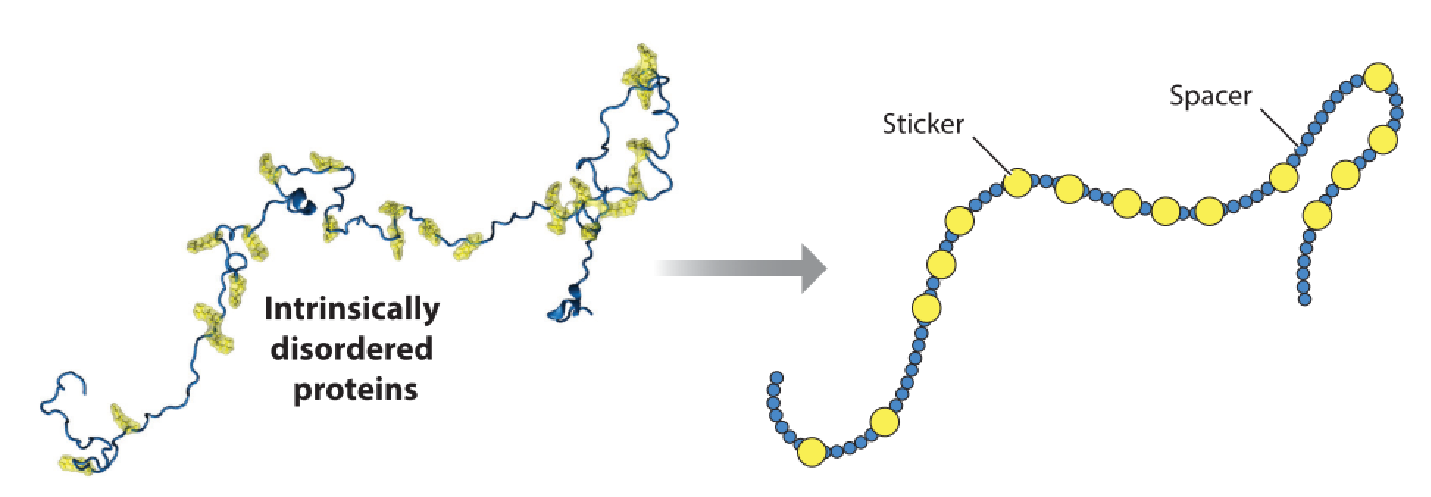
\includegraphics[width=1\linewidth]{figures/Figure8.1.pdf}
	\caption{Stickers-and-spacers model of condensate-forming intrinsically disordered proteins. Adapted from \cite{Choi2020}.}
	\label{fig:fig8.1}
\end{figure}

\noindent While the notion of phase separation has recently become relevant in biology to describe the behavior of associative polymers found in the cell \cite{Alberti2017}, such as proteins and RNAs, it appears to also fit well in modelling the behavior of FG-Nups. Both native and artificial FG-Nups have been shown to phase separate when present in physiological buffer above a certain critical concentration. Remarkably, the resulting droplets featured NPC-like selectivity \cite{Schmidt2015,Celetti2019,Ng2021}. 

Given such promising indications that a relatively simple framework can describe the complex multivalent interactions of FG-Nups, while conferring them with NPC-like selectivity, a few questions arise: (1) Can we pinpoint all the necessary and sufficient conditions that are needed for a protein to impart a NPC-like selective barrier? (2) Can we tune the `selective power' of a designer FG-mesh by varying simple parameters, such as the composition or distribution of the spacers and stickers? (3) How robust is the set of properties incorporated into the NupX sequence? 

To answer such questions, a possible approach could be to systematically vary some key parameters of a starting amino acid sequence and study the effects on its selective properties. From analysing the amino acid sequence of native FG-Nups  it can be observed that, just like in the stickers-and-spacers model, short sticky FG-motifs are separated by flexible, disorderd spacers \cite{Terry2009}. Having proven in Chapter \ref{chapter_4} that such a simple scheme is sufficient for building a selective protein, one may start altering parameters such as the spacer length, namely the distance between consecutive FG-repeats, or the physicochemical properties of the spacers by changing, \emph{e.g.}, their charge-to-hydropho\-bi\-ci\-ty ratio (C/H) (Fig.\ref{fig:fig8.2}). 

\begin{figure}[!htbp]
	\centering
	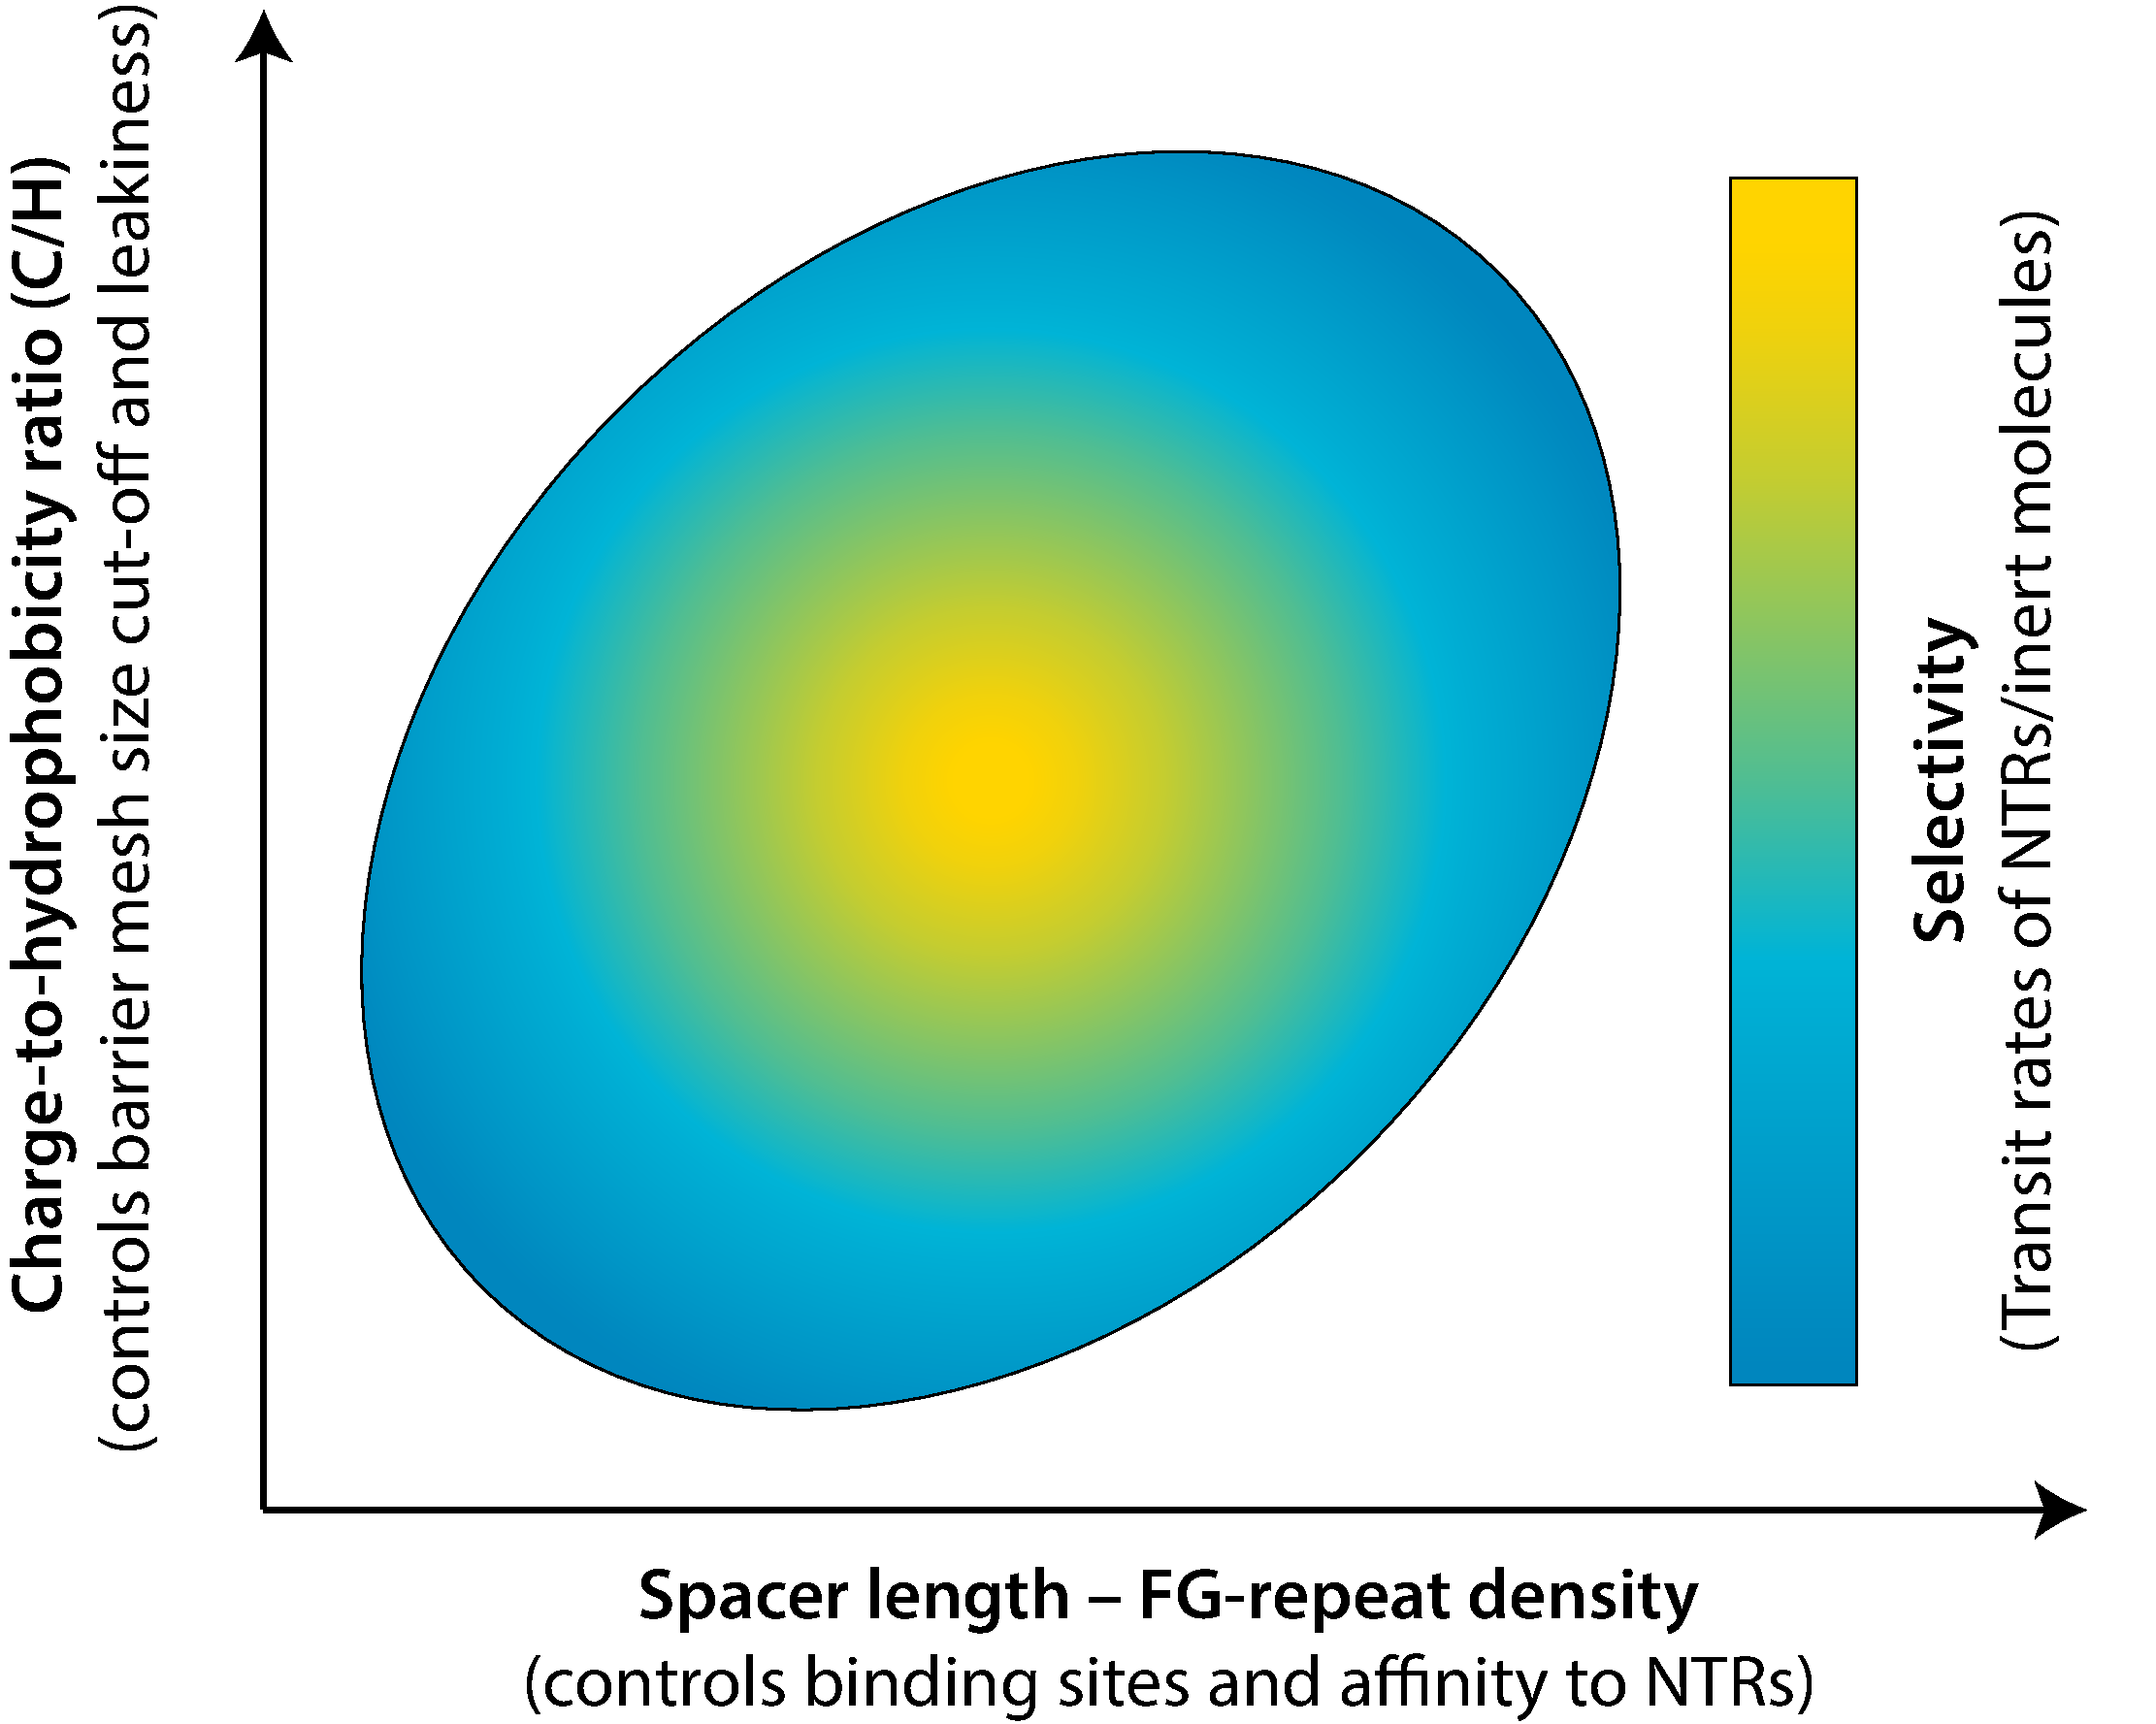
\includegraphics[width=0.9\linewidth]{figures/Figure8.2.pdf}
	\caption{Phase diagram for NPC selectivity as a function of spacer length and charge-to-hydrophobicity ratio (C/H).}
	\label{fig:fig8.2}
\end{figure}

\noindent Increasing the spacer length while keeping the C/H the same would result in a reduction of overall FG-repeats, namely a depletion of binding sites for transporter proteins like Kaps, which would, in principle, render the Kap partitioning into the FG-mesh less and less favorable. In this way, it would be possible to understand what spacer length is needed to achieve an efficient, energetically favorable permeation of transporters into the NPC. At the same time, changing the C/H of the spacers while keeping a fixed spacer length will modulate the overall cohesiveness of the FG-mesh. Increasing the C/H would indeed result in a looser mesh-size due to the more repulsive nature of the spacers, thereby diminishing the blocking capability of the FG-mesh while increasing the leakiness to larger cargoes. Acting independently on these two parameters may thus shed light on how the NPC central channel carries out its twofold function of transport facilitator (of cargo-bound NTRs) and size-selective molecular sieve (of inert molecules), ultimately explaining why FG-Nups have naturally evolved into their final sequences.

Ultimately, the capability to rationally design new proteins with tunable selective properties may enable the creation of molecular nanofilters for sample purification or selection and identification of specific biomarkers for diagnostics.

\section{Study how the Kaps regulate the FG-Nup barrier}
In Chapter \ref{chapter_7} we provided new compelling evidence that supports a recent model for nuclear transport, namely the Kap-centric model \cite{Lim2015}. Employing biomimetic nanopores reconstituted by grafting a native FG-Nup from yeast, Nsp1, to a solid-state nanopore, we explored the behavior of transporter Kap95 at increasing concentrations, finding that while a 'slow-phase' population of Kaps permanently resides in the pore, a 'fast-phase' is also present causing transient dips in the ionic current that correspond to fast ($\sim$ms) translocation events.

While such observations are insightful, we are left now with yet other questions: (1) Is there a preferential spatial  localization/segregation of slow-phase \emph{vs} fast-phase Kaps within the NPC channel? (2) Would Kaps behave the same in a more 'physiological' FG-mesh, composed by different types of FXFG- and GLFG-Nups, with the correct stoichiometry and positioning within the pore? (3) How do other transport factors (such as NTF2 or Mex67) enter into the Kap-centric picture? (4) While FG-Nups have been shown to phase separate in bulk solution forming micrometer-size gel-like particles, how does the presence of Kaps affects such phase state? 
\begin{figure}[!htbp]
	\centering
	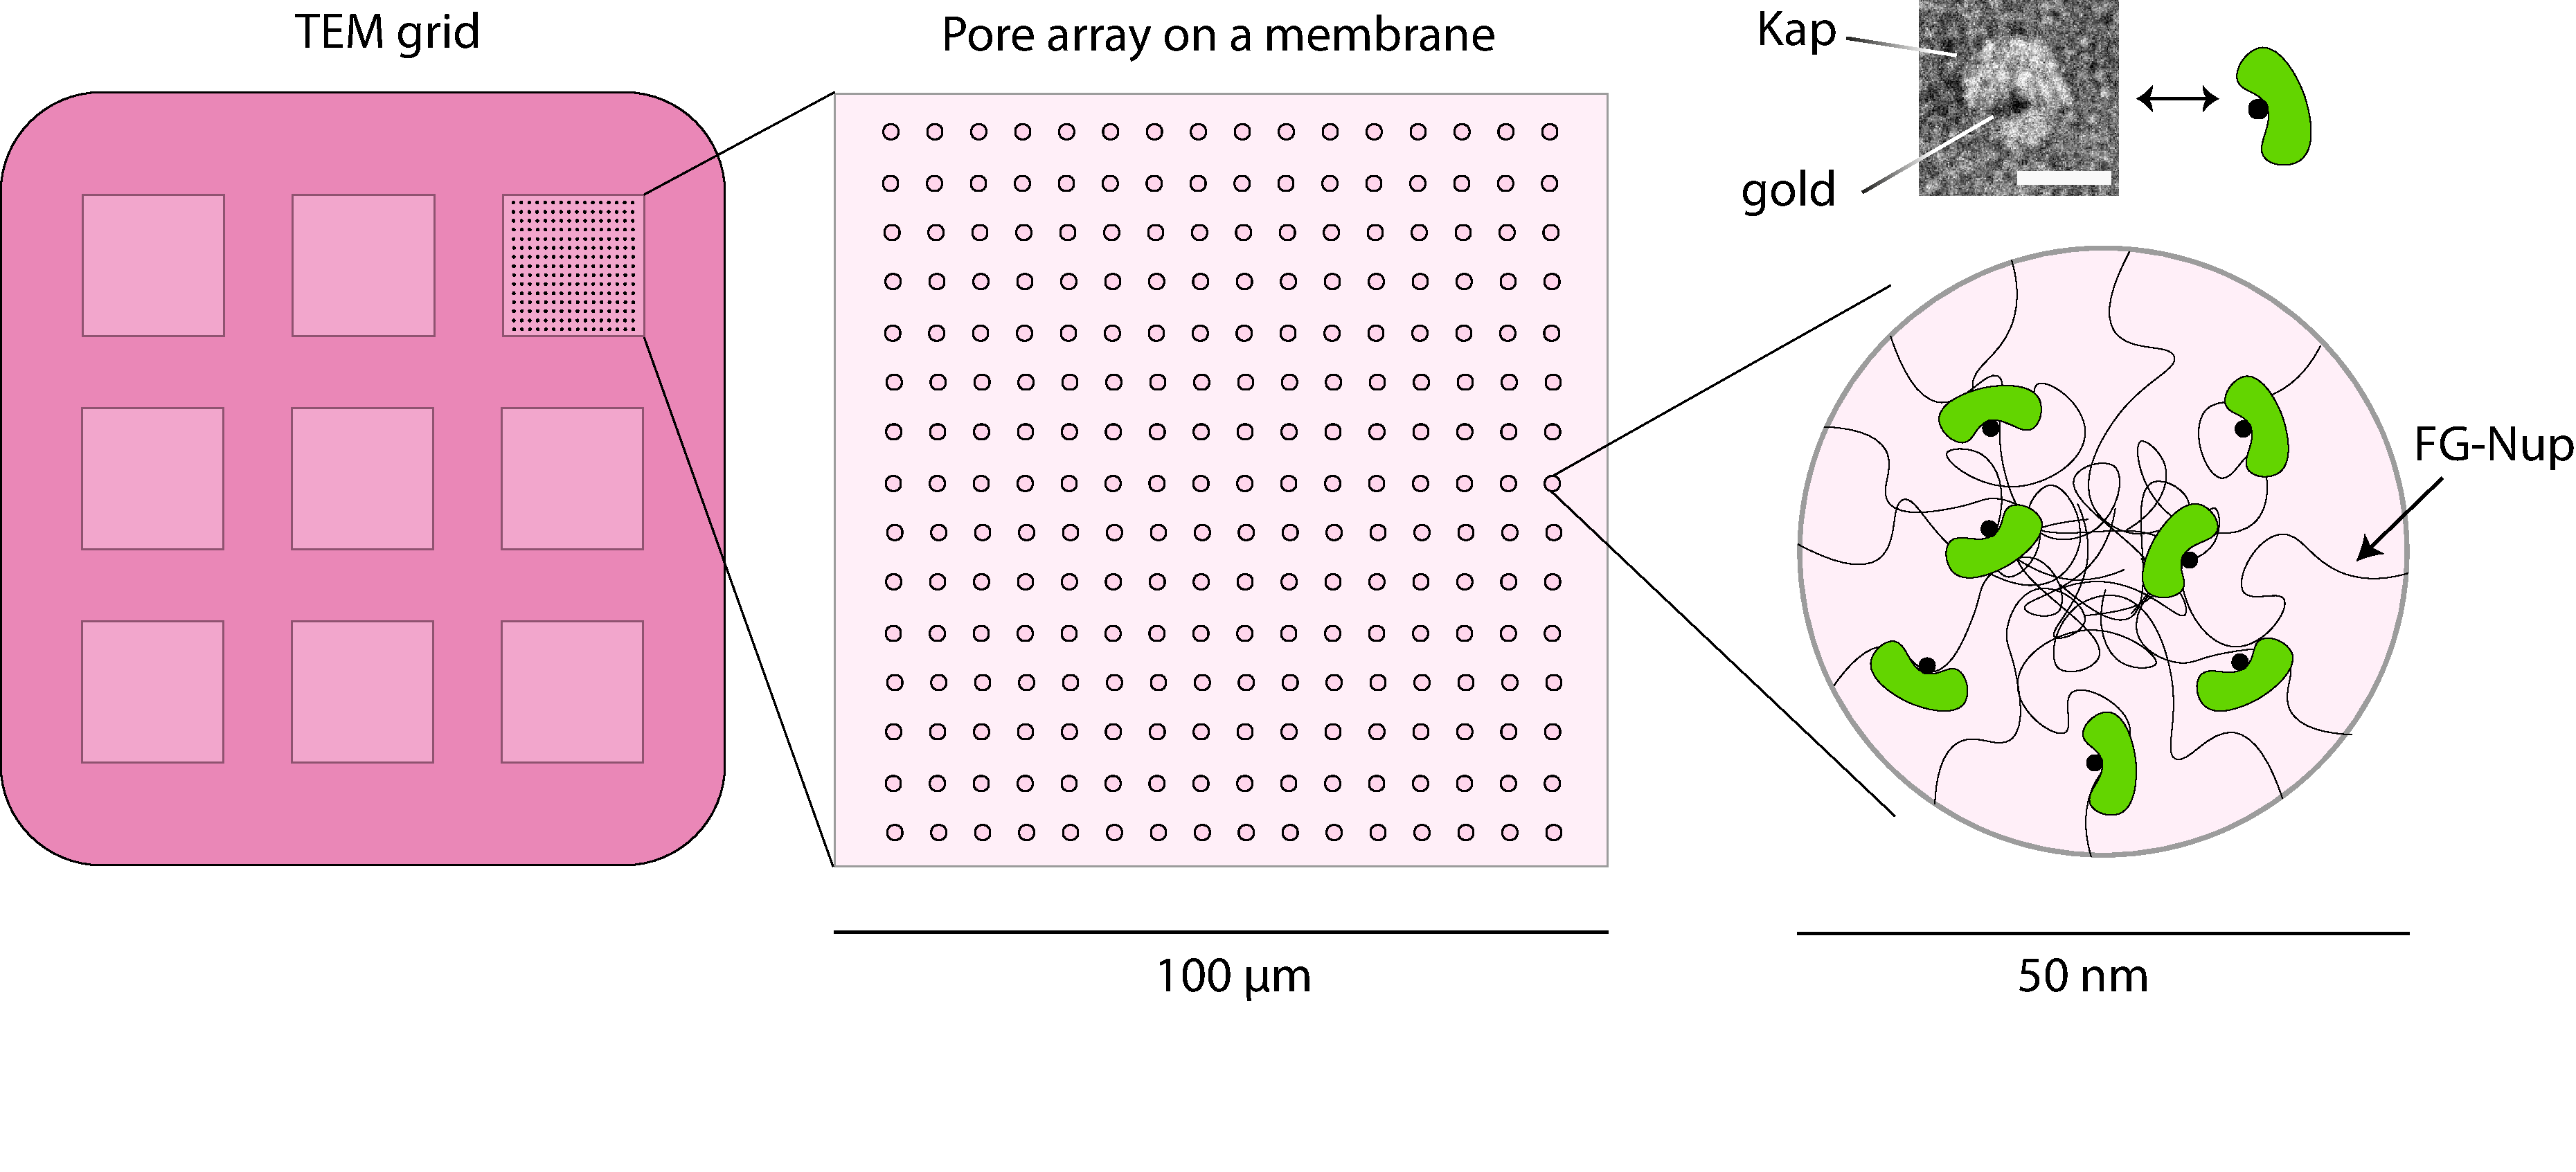
\includegraphics[width=1\linewidth]{figures/Figure8.3.pdf}
	\caption{CryoEM approach for resolving Kap localization within biomimetic nanopores. TEM micrograph on the top right shows a negative-staining image of a single Kap (white) bound to a 1.4 nm gold nanocluster. Scale bar: 10nm.}
	\label{fig:fig8.3}
\end{figure}
Although the ideal platform to answer all such questions would always be the real NPC, the astounding complexity of the cellular environment makes biomimetic NPCs still very attractive tools to probe the interaction between FG-Nups and NTRs. For instance, to test whether slow- and fast-phase Kaps are spatially segregated within the FG-mesh it would be possible to perform transmission electron microscopy in cryogenic conditions (cryoEM) of biomimetic nanopores, and resolve where Kaps reside in the pore (Fig.\ref{fig:fig8.3}). Detection of Kaps could be achieved by labelling them with tiny gold nanoclusters ($\sim$1-2 nm), whereas focused ion beam (FIB) \cite{Lanyon2007} or reactive ion etching (RIE) \cite{Verschueren2018} could be employed as high-throughput techniques to fabricate large pore arrays achieving thousands of pores in one single membrane. Given that slow-phase Kaps are expected to be constantly residing within the pore (nearly 100\% of the time), such population would result in a much higher signal (higher amount of gold particles) compared to the fast population which, in our biomimetic nanopores (Chapter \ref{chapter_7}), statistically occupies the pore for only <0.02\% of the time. By class-averaging over thousands of pores it would then be possible to build 2D (or even 3D by tilting the grid in TEM) probability distributions of where Kaps preferentially reside within the pore.

An alternative approach where the positioning and stoichiometry of FG-Nups can be achieved programmatically consists in using a DNA-origami scaffold (similar to the structure presented in Chapter \ref{chapter_5}) to spatially organize FG-Nups in a similar octagonal arrangement to the NPC (Fig.\ref{fig:fig8.4}) \cite{Ketterer2018,Fisher2018}.
\begin{figure}[!htbp]
	\centering
	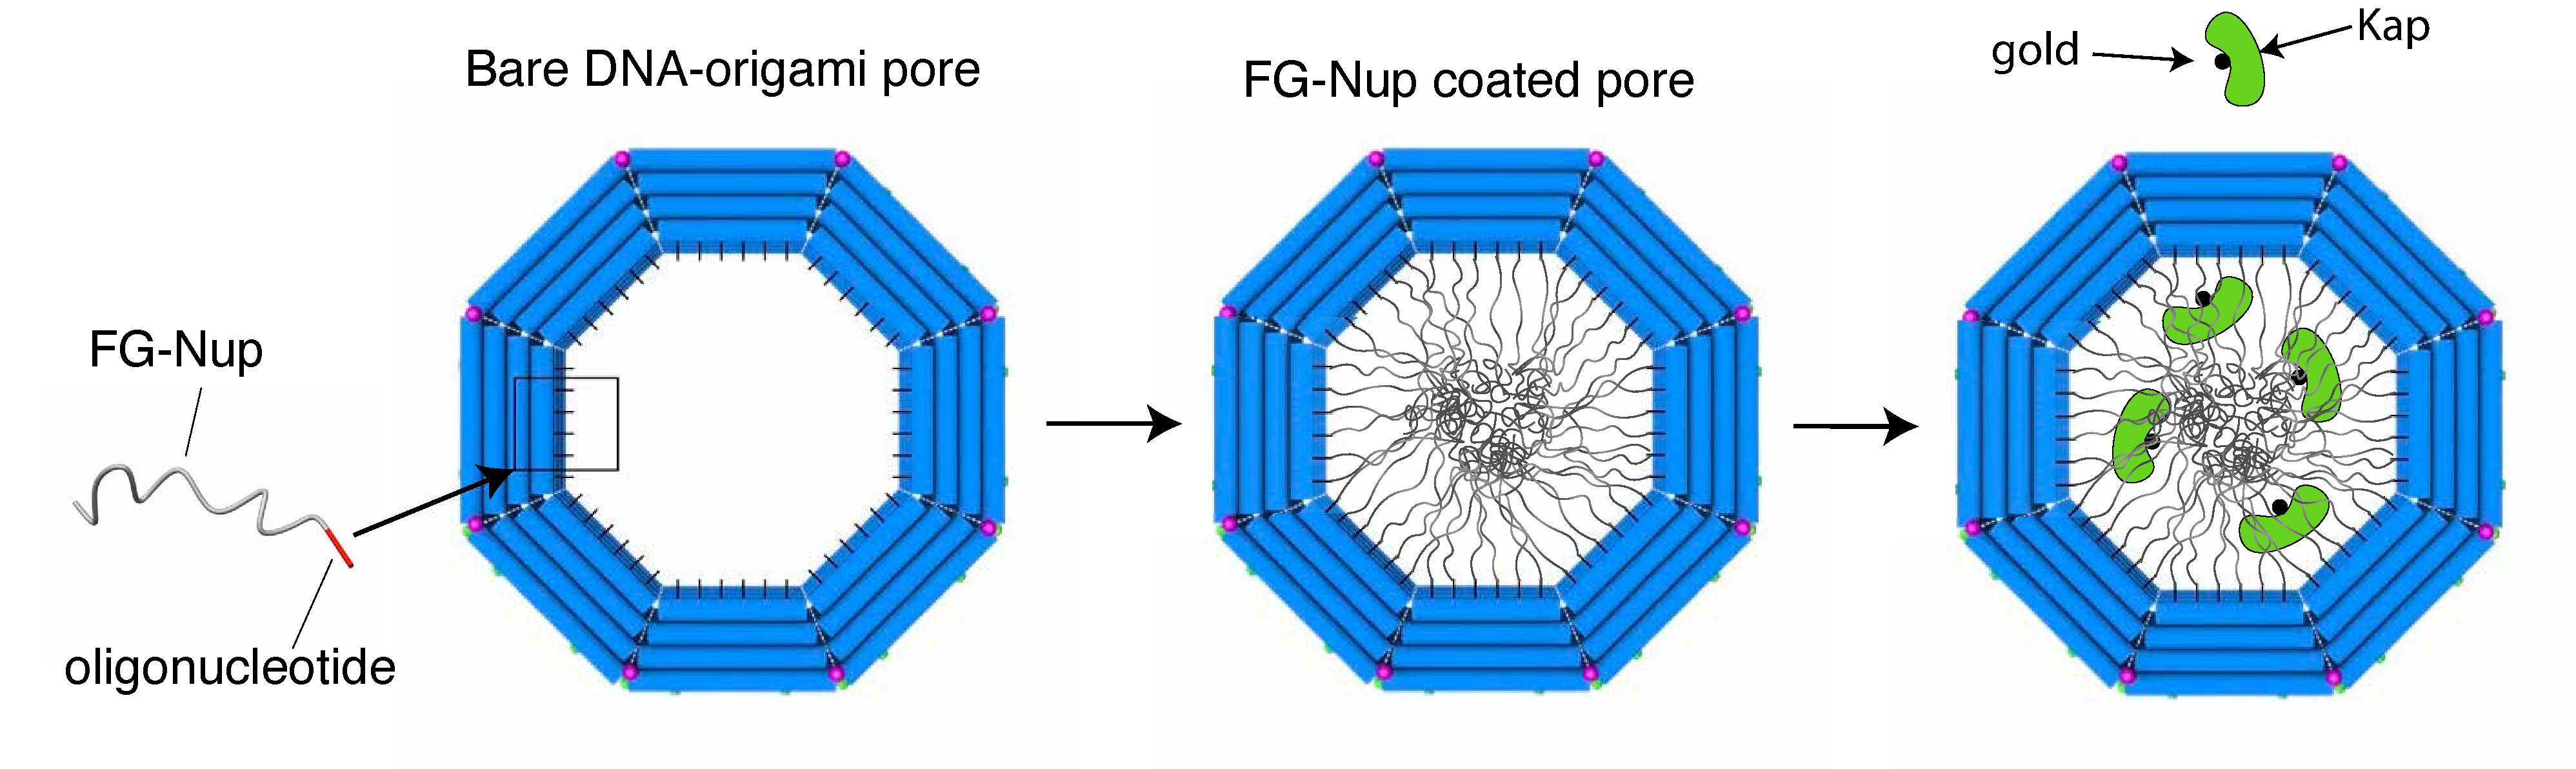
\includegraphics[width=1\linewidth]{figures/Figure8.4.pdf}
	\caption{Reconstitution of the FG-mesh using a DNA-origami scaffold and oligo-conjugated FG-Nups. Addition and localization of gold-labelled Kaps can be resolved with cryoEM imaging.}
	\label{fig:fig8.4}
\end{figure}
By combining such platform with cryoEM it would be possible to resolve the localization of gold-labelled Kaps within the reconstituted FG-mesh and study how they spatially organize within the pore when different types of FG-Nups, and combinations thereof, are present (Fig.\ref{fig:fig8.5}). This would provide new insights into how Kaps interact with a more physiological FG-mesh. 
\begin{figure}[!htbp]
	\centering
	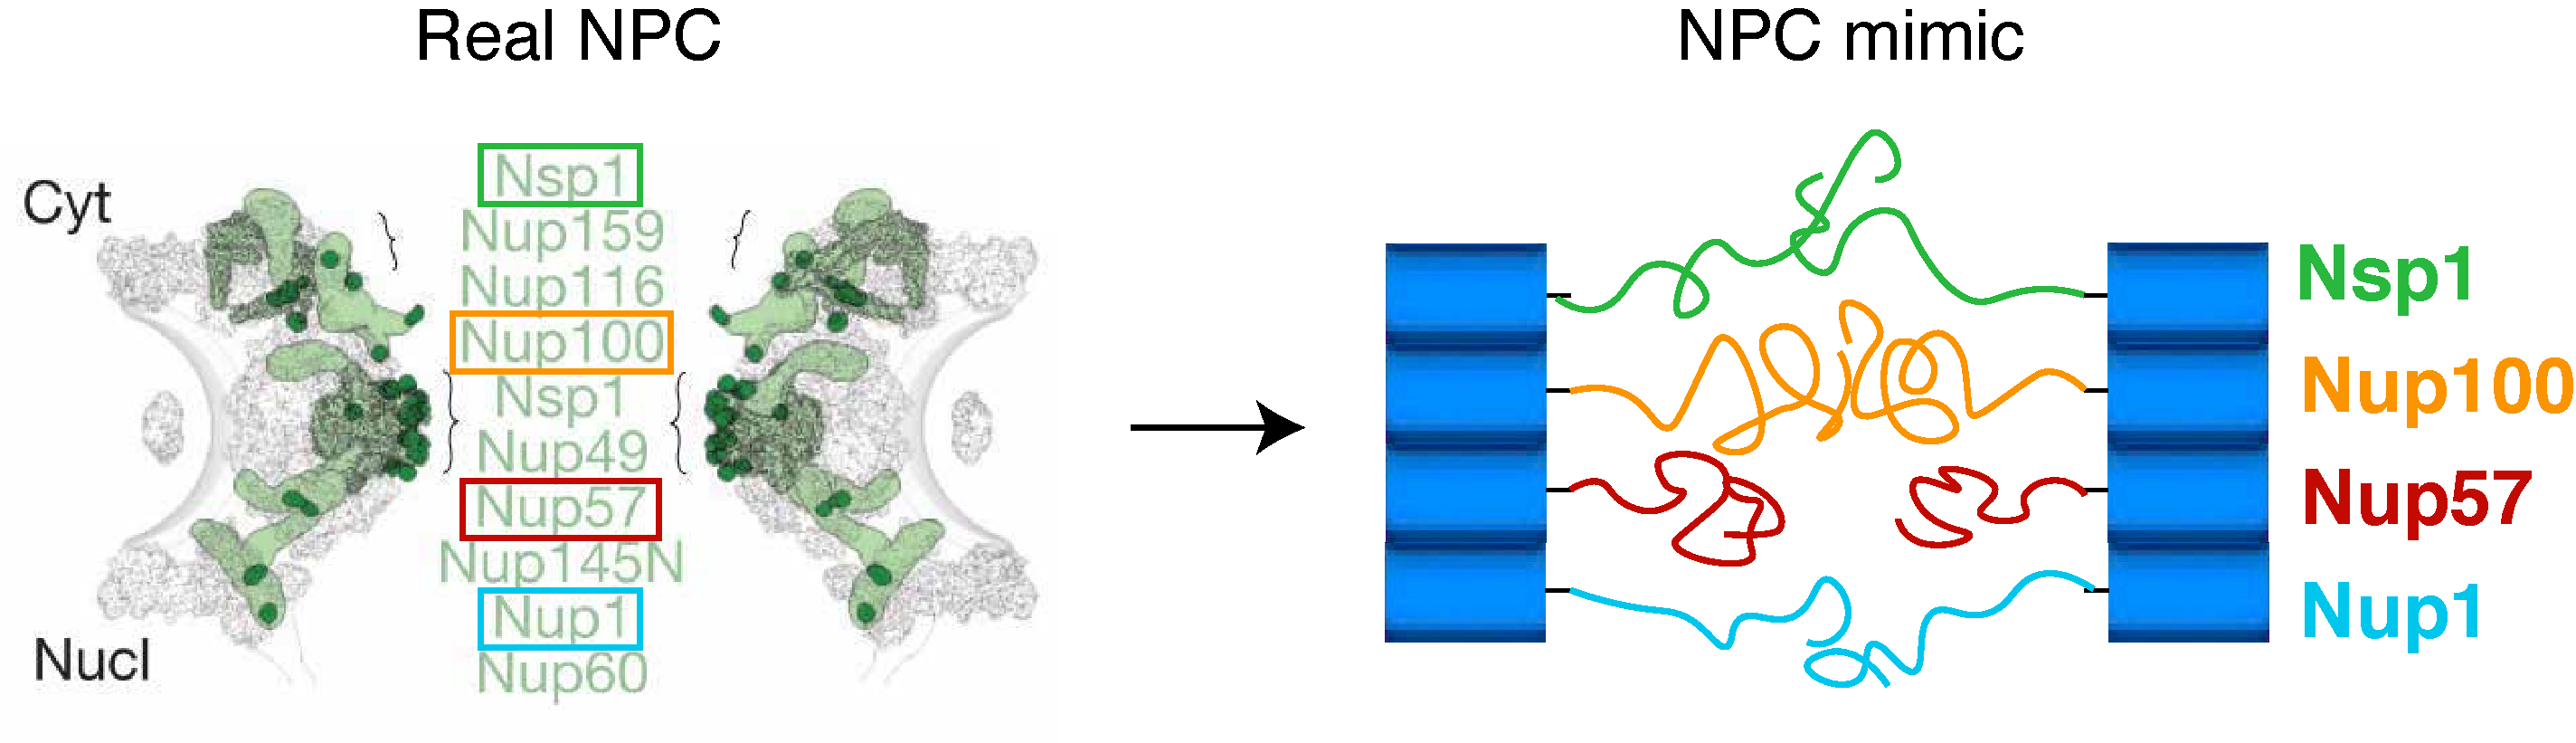
\includegraphics[width=0.9\linewidth]{figures/Figure8.5.pdf}
	\caption{Left: Illustration of the NPC scaffold (grey) with highlighted FG-Nup anchor domains (light green) and emanating points (dark green). Adapted from \cite{Kim2018}. Right: Side view of a FG-Nup coated DNA-origami scaffold with four different types of FG-Nups to mimic the FG-Nup distribution of the real NPC (left).}
	\label{fig:fig8.5}
\end{figure}

Probing how different transport factors such as NTF2 participate in such Kap-centric picture could be achieved with both suggested approaches by, for instance, labelling NTF2 with gold nanoparticles while leaving Kaps unlabelled in the background at physiological concentrations. By doing the reverse configuration (labelled Kaps, unlabelled NTF2) and subsequently overlaying the reconstructed spatial localization maps of both Kaps and NTF2 from independent experiments it would then be possible to observe whether a spatial segregation of different transporters occurs, as predicted in previous studies \cite{Davis2021,Wagner2015}. 

\noindent Another interesting approach may involve the use of biomimetic zero-mode-wave\-guide (ZMW) nanopores \cite{Klughammer2021} that are built by attaching FG-Nups to a nanopore made into a metal membrane (\emph{e.g.} gold or palladium). With this technique it would be possible to measure translocations through a biomimetic pore of fluorescently labelled proteins with different colors at  single-molecule resolution, thus allowing, unlike for standard electrical measurements, for parallel detection (multiplexing) of the various proteins within the same experiment. A number of key experiments could be performed on biomimetic ZMWs: (1) test how the presence of Kaps affects the transport efficiency of other transporters such as NTF2 or Mex67, hence addressing the hypothesis that Kaps can facilitate partitioning while speeding up transit times of the other NTRs through the NPC; (2) measure transport efficiency of differently sized inert molecules in the absence or presence of Kaps to assess whether and how Kaps play a role in strengthening the selective barrier; (3) Mimic the Kap-guided import process of cargo molecules and characterize the effect of RanGTP-induced cargo dissociation on the \emph{trans}-side of the pore with single-molecule resolution. Similarly, minimal export machineries based, \emph{e.g.}, on Mex67-RNA complexes could be tested as well.

Finally, characterizing FG-Nups condensates in the presence of Kaps and in the physiological FG-Nup-to-Kap stoichiometry, may shed light on the actual \emph{in vivo} phase state of the FG-mesh. Even better would be to characterize the phase of confined FG-Nups using biomimetic DNA-origami pores (built as in Fig.\ref{fig:fig8.4} and \ref{fig:fig8.5}), which could be achieved by fluorescently labelling different parts of the FG-Nup chain and measure the chain dynamics in real time using a F\"{o}rster resonance energy transfer (FRET) assay. Importantly, studying the behavior of FG-mesh dynamics and phase separation as a function of Kap concentration will bring new insights that may resolve the current discrepancies between the models of transport.

\section{Towards building an artificial nucleus}
In Chapter \ref{chapter_5} we presented a novel approach to insert large DNA-origami objects in the membrane of giant unilamellar vesicles using an inverted-emulsion technique (cDICE) \cite{Fragasso2021a}. The creation of large 30nm-passageways that span the membrane of a vesicle represents a significant step forward compared to previous works, where the largest DNA-origami pores ever formed across a lipid bilayer were at most 10nm-wide \cite{Iwabuchi2021,Thomsen2019}.

\noindent In the context of this thesis, an exciting application of this new development consists in functionalizing the origami pores with FG-Nups to reconstitute a NPC-like selective FG-mesh within the origami pore (Figures \ref{fig:fig8.4} and \ref{fig:fig8.5}), as it was similarly reported in previous works \cite{Ketterer2018,Fisher2018}. By combining the exquisite versatility and control that DNA-origami pores offer in terms of FG-Nup anchors positioning and distribution, together with our newly developed platform for embedding DNA-origami pores into a lipid membrane, it will be possible to recapitulate nuclear transport selectivity in a much more well-defined system.

A number of experiments that are of interest for the field of nuclear transport can be envisioned: (1) Characterizing how different combinations of FG-Nups impact the transport of NTRs and selectivity; (2) Testing whether the positioning of the different FG-Nups within the lumen, as is found in the real NPC, serves a particular task, such as creating an affinity gradient to impart a certain transport directionality for specific NTRs \cite{Pyhtila2003}; (3) Reconstitute a minimal nucleocytoplasmic transport cycle \emph{in vitro} by including NTRs, RanGTP/GDP gradient, together with cytoplasmic (RanGAP1) and nucleoplasmic (RanGEF) factors in the outer and inner compartment of the vesicle, respectively (Fig.\ref{fig:fig8.6}). Importantly, this would represent the first model of an artificial nucleus that may be used as an \emph{in vitro} mimic for studying nucleocytoplasmic transport.

\begin{figure}[!htbp]
	\centering
	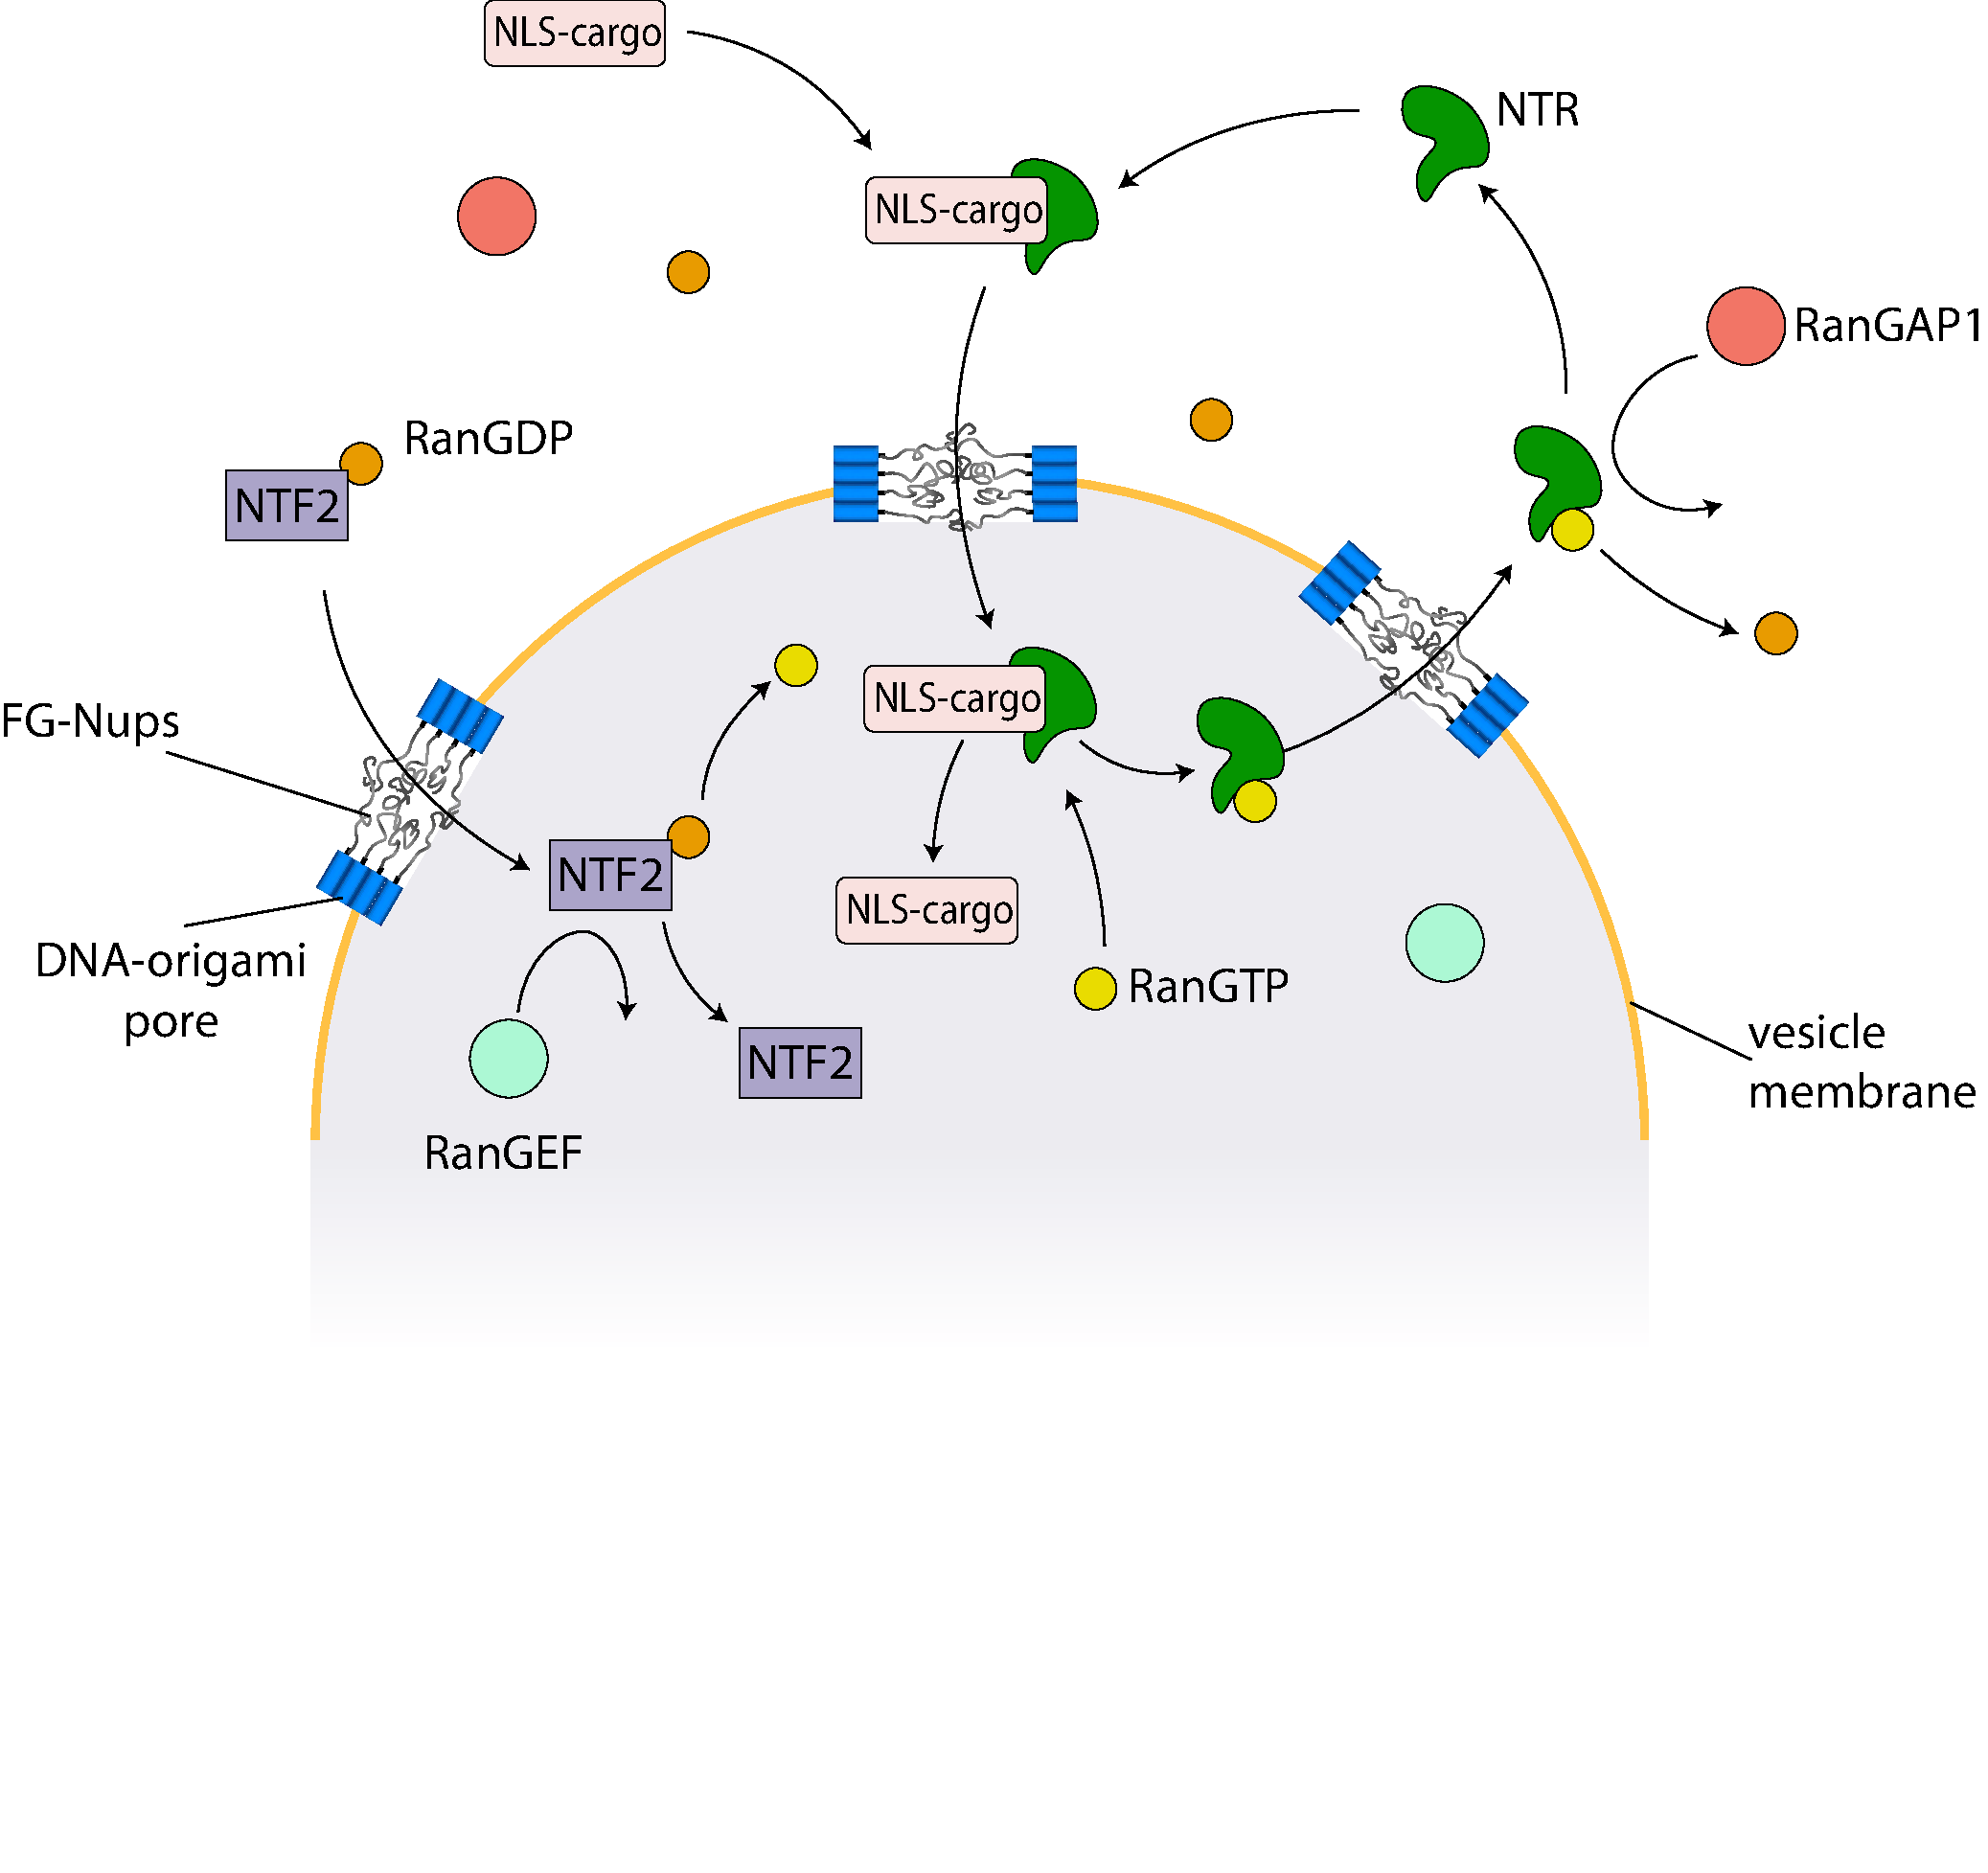
\includegraphics[width=1\linewidth]{figures/Figure8.6.pdf}
	\caption{Reconstitution \emph{in vitro} of nucleocytoplasmic transport in an artificial nucleus using biomimetic DNA-origami pores.}
	\label{fig:fig8.6}
\end{figure}

\section{Final outlook}
In the last two decades, the field of nuclear transport has seen a tremendous growth, from the `virtual gate' \cite{Rout2003} and `selective phase' models \cite{,Ribbeck2001,Ribbeck2002} being proposed in the early 2000s, which first speculated on the intrinsic mechanism underlying NPC selectivity, up to the most recent formulations of the Kap-centric model \cite{Kapinos2017a,Barbato*2020} where Kaps, together with the FG-Nups, assist in orchestrating the selective transport barrier. Notably, a great contribution to our understanding of the FG-Nup barrier and its interaction with Kaps has been provided by \emph{in vitro} techniques, where the FG-Nups are extracted from the cell and immobilized onto a surface or inside a nanopore, or let to phase-separate in bulk, with the aim to reconstitute and study a near-physiological system that mimics the NPC central channel. While a great deal of new information and insights have been produced over the years, there is still a lack of a general consensus as for how selective transport through the NPC proceeds mechanistically. Major outstanding questions pertain to: \\[0.5pt]

\noindent \textbf{What is the phase of the FG-mesh?}\\ A number of works have reported the tendency to phase-separate for the most cohesive FG-Nups, namely the native GLFG-Nups (Nup100 \cite{Schmidt2015}, Nup98 \cite{Schmidt2015}, Nup49 \cite{Celetti2019}) or a designer GLFG-Nup version \cite{Ng2021}, when these are present in physiological buffer beyond a certain critical concentration. Yet, it still doubtable whether such FG-Nup condensates are a good representation of the \emph{in vivo} FG-mesh. In fact, a number of non-negligible differences are present between such \emph{in vitro} system and \emph{in vivo}: (1) while FG-condensates are made from one single type of FG-Nup, \emph{e.g.} Nup100, the NPC features many different types of FG-Nups (11 in yeast \cite{Yamada2010}), which possess different amounts and types of FG-motifs, different physicochemical properties of the spacers, as well as varying lengths of the FG-domain. Importantly, an FG-mesh constituted by a more physiological FG-Nup composition may behave rather differently from a GLFG-Nup only condensate. (2) The geometry and well-defined organisation of FG-Nups in the NPC with FG-domains firmly anchored along the central lumen, is drastically different from a condensate where FG-Nups can freely diffuse around. Further studies should be carried out in order to characterize the phase state of more physiological FG-Nup mixtures.\\[0.1pt]

\noindent \textbf{What is the effect of Kaps on the FG-mesh?}\\ \emph{In vitro} experiments have shown that the interaction between Kaps and the FG-mesh can be broadly described as bimodal \cite{Eisele2010a, Kapinos2014,Kapinos2017a}, with a first Kap population binding strongly to the FG-mesh, while a second Kap population features fast association/dis\-sociation to the remaining FG-repeats. While such binding mechanism points to the presence of two distinct Kap populations in the real NPC (fast and slow phases), the effect of Kaps on the phase state and spatial arrangement of the real FG-mesh is still poorly understood. Indeed, given that phase separation is driven by FG-FG interactions \cite{Frey2006}, and the fact that Kaps bind FG-repeats as well, there may be a regime (\emph{e.g.}, at high enough Kap concentration) where Kaps sequester enough FG-repeats that cause the dissolution of the condensate. Experiments targeted to drawing a phase diagram for FG-Nups phase behavior at varying Kap concentrations are essential to understand the real phase of the \emph{in vivo} FG-mesh and ultimately discriminate among the current models of transport. \\[0.1cm]

\noindent \textbf{What is the spatial distribution of the different FG-Nups and NTRs?}\\
Finally, open questions also revolve around the presence of distinct, spatially segregated regions within the NPC central channel, which may originate from a number of contributions: (1) The structure of the NPC scaffold is far from being a perfect cylinder (Figure \ref{fig:fig8.5}, left), but rather consists of a hour-glass shaped structure \cite{Kim2018}. Together with the asymmetrical distribution of the different FG-Nups along the channel length, this may result in a heterogenous distribution of protein mass and FG-repeat density along the channel with effects on nuclear transport that are still unexplored \cite{Kim2018}; (2) The heterogeneous, often bimodal \cite{Yamada2010}, amino acid composition of FG-Nups may as well lead to regions with higher or lower density in terms of both protein mass and FG-repeat density. This may in turn result in different pathways to facilitate the transport of different NTRs and inert molecules \cite{Yamada2010};
(3) Finally, the arrangement and density distribution of the FG-mesh should also account for the presence of NTRs, which may alter the overall conformation and phase behavior of the FG-Nup barrier. Furthermore, as binding affinities between NTRs and FG-Nups vary widely depending on the specific NTR or FG-Nup \cite{Pyhtila2003}, spatial segregation effects of the different NTRs, such as Kaps \emph{vs} NTF2 \cite{Davis2021,Wagner2015}, or even from the same NTR class, \emph{e.g.} slow-phase vs fast-phase Kaps \cite{Kapinos2014}, within the NPC central channel may occur.\\[0.1pt]

\noindent Aside for being a fascinating subject of investigation for many scientists, nuclear transport constitutes a vital process for the survival of the cell. In fact, functional impairment of nucleoporins has been associated with a number of disorders, from various forms of cancer \cite{Cronshaw2004}, to autoimmune diseases \cite{Duarte-Rey2012}. Understanding NPC function mechanism in greater detail will ultimately aid in developing effective treatments for such diseases.

\references{chapter-8/chapter-8}
